
% Eigener Beitrag: Beschreibung, Begründung, Aufzeigung, Methode, Fazit

\chapter{Anforderungen und Analyse}
\label{sec:analyse}
In diesem Kapitel werden die technischen Aspekte der API der travelwindow AG beschrieben, sowie die eingesetzte BPMN Software beschrieben.

\section{Anaylse der travelwindow AG API}
\label{sec:analyse:api}
Die \Gls{glos:api} der travelwindow AG ist mit \Gls{glos:hal} aufgebaut. Sprich es gibt einen Einstiegspunkt, welcher unter "`/"' erreichbar ist. Danach navigiert man sich über Links durch die Schnittstelle durch. Dies macht die API frei erkundbar, jedoch die Umsetzung mittels BPMN komplexer.

Nachfolgend werden die benötigten Anfragen an die API aufgeführt, welche für die Suche eines Hotel und Flug Angebotes benötigt werden (siehe \cref{sec:Recherche:rahmenbedingungen:prozesse} \nameref{sec:Recherche:rahmenbedingungen:prozesse}). Die aufgeführten Antworten sind für eine bessere Übersichtlichkeit verkürzt.


\begin{lstlisting}[language=json,firstnumber=1]
{
	"href": "https://dev-api.travel.ch/",
	[...]
	"hotelPlusFlightSearch":{ "href": "https://dev-api.travel.ch/HotelPlusFlight/Search" },
	[...]
}
\end{lstlisting}
Dies ist die Root Ressource. Das Feld hotelPlusFlightSearch ist der Einstigspunkt für die Hotel und Flug Suche.

\begin{lstlisting}[language=json,firstnumber=1]
{
  "href":"https://dev-api.travel.ch/HotelPlusFlight/Search",
  "form":{
    "description": {"href":"https://dev-api.travel.ch/HotelPlusFlight/SearchFormDescription/HotelPlusFlight"},
    "submit":{
      "href":"https://dev-api.travel.ch/HotelPlusFlight/Search{?destination,periodOfStay,roomOccupancies*,departureAirport,departureAirports*,targetPeriodOfStay,hotelCategories*,ratings,mealTypeCategories*,directFlight,flightClasses*,matchHotels,productType}"
    },
    "data":{ [...] },
    "alternatives":null
  },
  "results":null
}
\end{lstlisting}
/HotelPlusFlight/Search führt eine Suche aus. Wird die Ressource jedoch wie hier ohne Parameter aufgerufen, so sind keine Suchresultate definiert.
Hier wird auch beschrieben, wie eine Suche ausgeführt werden kann. Im Feld form->submit ist die \gls{url} definiert, welche für eine Suche aufgerufen werden muss. Bei dieser sind jedoch Parameter zwingend, welche in der SearchFormDescription unter form->description weiter beschrieben werden.

\begin{lstlisting}[language=json,firstnumber=1]
{
  "href":"https://dev-api.travel.ch/HotelPlusFlight/SearchFormDescription/HotelPlusFligh",
  "destination":{
    "type":{ "href":"https://dev-api.travel.ch/FieldType/Destination" },
    "config":{
      "suggestUri":{ "href":"https://dev-api.travel.ch/DestinationSuggestions/HotelPlusFligh?q=%7B_%7D" }
    }
  },
  "periodOfStay":{
    "type":{ "href":"https://dev-api.travel.ch/FieldType/PeriodOfStay" },
    "config":{
      "minCheckInDate":"2016-06-16",
      "maxCheckInDate":"2017-06-16",
      "minNumberOfNights":1,
      "maxNumberOfNights":90
    }
  },
  "roomOccupancies":{
    "type":{ "href":"https://dev-api.travel.ch/FieldType/RoomOccupancies" },
    "config":{
      "minRooms":1,
      "maxRooms":2,
      "minAdultsPerRoom":1,
      "maxAdultsPerRoom":6,
      "minChildrenPerRoom":0,
      "maxChildrenPerRoom":4,
      "minChildAge":0,
      "maxChildAge":18
    }
  },
  "departureAirport":{
    "type":{ "href":"https://dev-api.travel.ch/FieldType/Airport" },
    "config":[
      { "href":"https://dev-api.travel.ch/Destination/A6299466" },
      { "href":"https://dev-api.travel.ch/Destination/A6299720" },
      { "href":"https://dev-api.travel.ch/Destination/A2660644" },
      { "href":"https://dev-api.travel.ch/Destination/A6299722" },
      { "href":"https://dev-api.travel.ch/Destination/A3208823" },
      { "href":"https://dev-api.travel.ch/Destination/A3174133" }
    ]
  },
  [...]
}
\end{lstlisting}
Dies ist die SearchFormDescription für die Hotel und Flug Suche. Sie beschreibt die Parameter, welche für eine Suche benutzt werden können.

\begin{lstlisting}[language=json,firstnumber=1]
{
  "href":"https://dev-api.travel.ch/HotelPlusFlight/Search?destination=https%3A%2F%2Fdev-api.travel.ch%2FDestination%2F6547539&periodOfStay.checkInDate=2016-10-05&periodOfStay.checkOutDate=2016-10-08&[...]",
  "form":{
    [...]
    "data":{
      "destination":{ "href":"https://dev-api.travel.ch/Destination/6547539" },
      "periodOfStay":{
        "checkInDate":"2016-10-05",
        "checkOutDate":"2016-10-08"
      },
      [...]
      "roomOccupancies":[
        { "dateOfBirths":[ null, null ] }
      ],
      "departureAirport":{ "href":"https://dev-api.travel.ch/Destination/A6299722" },
      [...]
    },
    "alternatives":null
  },
  "results":{
    "href":"https://dev-api.travel.ch/HotelPlusFlight/SearchResultPage/19E2B6BB-1F06-4396-B86E-169EDB368B0E?hotelCategories%5B0%5D=https%3A%2F%2Fdev-api.travel.ch%2FHotelCategory%2FNone[...]"
  }
}
\end{lstlisting}
Bei dieser Anfrage handelt es sich um eine Suche, dieses mal mit Suchparametern. Das Feld results ist nun mit einer SearchResultPage befüllt.

\begin{lstlisting}[language=json,firstnumber=1]
{
  "href":"https://dev-api.travel.ch/HotelPlusFlight/SearchResultPage/19E2B6BB-1F06-4396-B86E-169EDB368B0E?sortMethod.type=https%3A%2F%2Fdev-api.travel.ch%2FSortType%2FPrice&ratings.minimal=0[...]",
  "citytripSearch":{
    "href":"https://dev-api.travel.ch/HotelPlusFlight/Search?destination=https%3A%2F%2Fdev-api.travel.ch%2FDestination%2F6547539&periodOfStay.checkInDate=2016-10-05&periodOfStay.checkOutDate=2016-10-08[...]"
  },
  "form":{
    "description":{
      "href":"https://dev-api.travel.ch/HotelPlusFlight/SearchResultPageFormDescription/19E2B6BB-1F06-4396-B86E-169EDB368B0E?searchResultPageId=E5241069-1272-4DD0-946E-46DD2E9D55E6"
    },
    "data":{ [...] },
    "facets":{ [...] },
    "submit":{
      "href":"https://dev-api.travel.ch/HotelPlusFlight/SearchResultPage/19E2B6BB-1F06-4396-B86E-169EDB368B0E{?paging.offset,paging.size,[...],luggageOptions*}"
    },
    "alternatives":null
  },
  "teaserForm":{ [...] },
  "totalCount":263,
  "count":263,
  "results":{
    "href":"https://dev-api.travel.ch/HotelPlusFlight/SearchResults/E5241069-1272-4DD0-946E-46DD2E9D55E6"
  },
  "mapFeatures":{
    "href":"https://dev-api.travel.ch/HotelPlusFlight/SearchResultPage/E5241069-1272-4DD0-946E-46DD2E9D55E6/Map"
  }
}
\end{lstlisting}
Dies ist die SearchResultPage. Auf travel.ch wird diese verwendet, um die Resultate weiter zu filtrieren. Dies ist jedoch bei diesem Projekt nicht vorgesehen. Von dieser Anfrage wird nur das Feld results benötigt, welches die Suchresultate beinhaltet.

\begin{lstlisting}[language=json,firstnumber=1]
{
  "href":"https://dev-api.travel.ch/HotelPlusFlight/SearchResults/E5241069-1272-4DD0-946E-46DD2E9D55E6",
  "items":[
    {
      "href":"https://dev-api.travel.ch/HotelPlusFlight/SearchResult/21ca65ff-976a-4a3e-bc92-b17608db3b25?pageId=58B8D81D-12B5-4EEE-9CE9-902CCDF01791",
      "citytripSearchResultPage":{
        "href":"https://dev-api.travel.ch/HotelPlusFlight/SearchResultPage/19E2B6BB-1F06-4396-B86E-169EDB368B0E?paging.offset=0&paging.size=12&sortMethod.type=https%3A%2F%2Fdev-api.travel.ch%2FSortType%2FPrice[...]"
      },
      "hotelInformation":{
        "href":"https://dev-api.travel.ch/HotelInformation/DDA48396-8105-433D-B75B-668F96EC89D8"
      },
      "offer":{
        "href":"https://dev-api.travel.ch/HotelPlusFlight/Offer?destination=https%3A%2F%2Fdev-api.travel.ch%2FDestination%2FH_63CA0931EAD8A33EF988144360A8056C&offerHotelInformation=https%3A%2F%2Fdev-api.travel.ch%2FHotelInformation%2FDDA48396-8105-433D-B75B-668F96EC89D8[...]",
        "price":{
          "actualTotal":{
            "amount":45512,
            "currency":{ "href":"https://dev-api.travel.ch/Currency/CHF" }
          },
          "previousTotal":null,
          "averagePrice":{
            "type":{ "href":"https://dev-api.travel.ch/AveragePriceType/PerPerson" },
            "value":{
              "amount":22800,
              "currency":{ "href":"https://dev-api.travel.ch/Currency/CHF" }
            }
          }
        }
      },
      "availability":null,
      "labels":null,
      "distanceInMeters":null
    },
    [...]
  ]
}
\end{lstlisting}
Das sind die Hotelresultate der Suche. Diese Antwort ist sehr verkürzt. Es wird nur ein Resultat hier angezeigt um die Übersicht zu behalten.



\begin{lstlisting}[language=json,firstnumber=1]
{
  "href":"https://dev-api.travel.ch/HotelInformation/dda48396-8105-433d-b75b-668f96ec89d8",
  "name":"Generator Berlin Prenzlauer Berg",
  "descriptions":{
    "href":"https://dev-api.travel.ch/HotelInformation/dda48396-8105-433d-b75b-668f96ec89d8/Descriptions",
    "hotel":{ "href":"https://dev-api.travel.ch/HotelInformation/dda48396-8105-433d-b75b-668f96ec89d8" },
    "items":[
      {
        "type":{ "href":"https://dev-api.travel.ch/HotelDescriptionType/Hotel" },
        "text":"Das Stadthotel ist in einem futuristischen Design erbaut und befindet sich in der Naehe der Berlin Arena und der S-Bahnstation Landsberger Allee, nur sechs Strassenbahnhaltestellen vom Alexanderplatz entfernt. Das stilvolle Hostel verfuegt ueber farbenfrohe Zimmer mit Schliessfach und eigenem Bad bzw. Gemeinschaftsbad und die Bar organisiert taegliche Veranstaltungen und woechentliche Partys. Darueber hinaus werden Karaoke-Abende, Filmvorfuehrungen und kostenlose Wanderungen angeboten. Dieses Hostel verspricht einen einzigartigen und unvergesslichen Aufenthalt."
      }
    ]
  },
  "images":{
    "href":"https://dev-api.travel.ch/HotelInformation/dda48396-8105-433d-b75b-668f96ec89d8/ImageGallery",
    "hotel":{ "href":"https://dev-api.travel.ch/HotelInformation/dda48396-8105-433d-b75b-668f96ec89d8" },
    "main":{
      "href":"https://dev-api.travel.ch/HotelInformation/dda48396-8105-433d-b75b-668f96ec89d8/Image/SG90ZWxcRERBNFw4Mzk2LTgxMDUtNDMzRC1CNzVCLTY2OEY5NkVDODlEOFwwMTU5NzVhX2hiX2JhXzAxMi5qcGc=",
      "url":"//dev-images.travel.ch/pictures/Hotel/DDA4/8396-8105-433D-B75B-668F96EC89D8/015975a_hb_ba_012.jpg",
      "alt":null,
      "description":null
    },
    "items":[
      {
        "href":"https://dev-api.travel.ch/HotelInformation/dda48396-8105-433d-b75b-668f96ec89d8/Image/SG90ZWxcRERBNFw4Mzk2LTgxMDUtNDMzRC1CNzVCLTY2OEY5NkVDODlEOFwwMTU5NzVhX2hiX2JhXzAxMi5qcGc=",
        "url":"//dev-images.travel.ch/pictures/Hotel/DDA4/8396-8105-433D-B75B-668F96EC89D8/015975a_hb_ba_012.jpg",
        "alt":null,
        "description":null
      },
      {
        "href":"https://dev-api.travel.ch/HotelInformation/dda48396-8105-433d-b75b-668f96ec89d8/Image/SG90ZWxcRERBNFw4Mzk2LTgxMDUtNDMzRC1CNzVCLTY2OEY5NkVDODlEOFwwMTU5NzVhX2hiX2xfMDA5LmpwZw==",
        "url":"//dev-images.travel.ch/pictures/Hotel/DDA4/8396-8105-433D-B75B-668F96EC89D8/015975a_hb_l_009.jpg",
        "alt":null,
        "description":null
      },
      [...]
    ]
  },
  "facts":{
    "href":"https://dev-api.travel.ch/HotelInformation/dda48396-8105-433d-b75b-668f96ec89d8/Facts",
    "hotel":{
      "href":"https://dev-api.travel.ch/HotelInformation/dda48396-8105-433d-b75b-668f96ec89d8"
    },
    "items":[
      {
        "type":{ "href":"https://dev-api.travel.ch/FactGroupType/Environment" },
        "facts":[
          {
            "type":{ "href":"https://dev-api.travel.ch/FactType/Simple" },
            "data":"Busbahnhof/Bahnhof 3500 m"
          },
          {
            "type":{ "href":"https://dev-api.travel.ch/FactType/Simple" },
            "data":"Vergnuegungsviertel 3500 m"
          },
        ]
      },
      {
        "type":{ "href":"https://dev-api.travel.ch/FactGroupType/Hotel" },
        "facts":[
          {
            "type":{ "href":"https://dev-api.travel.ch/FactType/Simple" },
            "data":"NO Haustiere auch ueber 5 kg erlaubt"
          },
          {
            "type":{ "href":"https://dev-api.travel.ch/FactType/Simple" },
            "data":"Waescherei"
          },
          [...]
        ]
      },
      {
        "type":{ "href":"https://dev-api.travel.ch/FactGroupType/Room" },
        "facts":[
          {
            "type":{ "href":"https://dev-api.travel.ch/FactType/Simple" },
            "data":"NO Raucherzimmer"
          },
          {
            "type":{ "href":"https://dev-api.travel.ch/FactType/Simple" },
            "data":"Dusche"
          },
          [...]
        ]
      }
    ]
  },
  "ratings":null,
  "geoLocation":{
    "type":"Point",
    "coordinates":[ 13.455673, 52.529681 ]
  },
  "destination":{ "href":"https://dev-api.travel.ch/Destination/H_63CA0931EAD8A33EF988144360A8056C" },
  "keyFacts":[
    { "href":"https://dev-api.travel.ch/KeyFact/Bar" },
    { "href":"https://dev-api.travel.ch/KeyFact/WLAN" }
  ],
  "labels":[
    { "href":"https://dev-api.travel.ch/Label/CustomerRecommendation" }
  ],
  "hotelCategory":{ "href":"https://dev-api.travel.ch/HotelCategory/One" },
  "addressLines":[ "10407 Prenzlauer Berg", "Deutschland" ],
  "tourOperator":null,
  "tourOperatorGtcUrl":null
}
\end{lstlisting}
Jedes Suchresultat der vorherigen Anfrage beinhaltet eine solche (oben) HotelInformation. Diese beherbergt alle Informationen eines Hotels, die nicht an ein Angebot gebunden ist. Zum Beispiel Bilder, Beschreibungen, etc. Was nicht enthalten ist sind Preise.



\begin{lstlisting}[language=json,firstnumber=1]
{
  "href":"https://dev-api.travel.ch/HotelPlusFlight/Offer?destination=https%3A%2F%2Fdev-api.travel.ch%2FDestination%2FH_9675C54E32056B7DC2393EE1D758FEB9&offerHotelInformation=https%3A%2F%2Fdev-api.travel.ch%2FHotelInformation%2F46FFEA61-6A24-4FCB-AE6A-524CE6E752DF[...]",
  "tourOperator":{ "href":"https://dev-api.travel.ch/TourOperator/TWCH" },
  "form":{
    "data":{
      "destination":{ "href":"https://dev-api.travel.ch/Destination/H_9675C54E32056B7DC2393EE1D758FEB9" }
    }
  },
  "selectForm":{ [...] },
  "hotelForm":{
    "description":{ "href":"https://dev-api.travel.ch/HotelPlusFlight/HotelConfigurationFormDescription?offerHotelInformation=https%3A%2F%2Fdev-api.travel.ch%2FHotelInformation%2F46FFEA61-6A24-4FCB-AE6A-524CE6E752DF[...]" },
    [...]
  },
  "flightForm":{
    "description":{ "href":"https://dev-api.travel.ch/HotelPlusFlight/FlightConfigurationFormDescription?offerHotelInformation=https%3A%2F%2Fdev-api.travel.ch%2FHotelInformation%2F46FFEA61-6A24-4FCB-AE6A-524CE6E752DF&roomOccupancies%5B0%5D.dateOfBirths%5B0%5D=null[...]" },
    [...]
  },
  "orderForm":{
    "description":{ "href":"https://dev-api.travel.ch/HotelPlusFlight/OrderFormDescription" },
    "submit":{"href":"https://dev-api.travel.ch/HotelPlusFlight/SearchResult/Offer/Order?destination=https%3A%2F%2Fdev-api.travel.ch%2FDestination%2FH_9675C54E32056B7DC2393EE1D758FEB9&offerHotelInformation=https%3A%2F%2Fdev-api.travel.ch%2FHotelInformation%2F46FFEA61-6A24-4FCB-AE6A-524CE6E752DF[...]",
      "action":"POST"
    }
  },
  "price":{
    "actualTotal":{
      "amount":174370,
      "currency":{ "href":"https://dev-api.travel.ch/Currency/CHF" }
    },
    "previousTotal":null,
    "averagePrice":{
      "type":{ "href":"https://dev-api.travel.ch/AveragePriceType/PerPerson" },
      "value":{
        "amount":87200,
        "currency":{ "href":"https://dev-api.travel.ch/Currency/CHF" }
      }
    }
  },
  "travelPeriod":{
    "startDate":"2016-10-05",
    "endDate":"2016-10-12"
  },
  "hotelInformation":{ "href":"https://dev-api.travel.ch/HotelInformation/46FFEA61-6A24-4FCB-AE6A-524CE6E752DF" },
  "transfer":{ "href":"https://dev-api.travel.ch/HotelPlusFlight/Transfer/NotIncluded" }
}
\end{lstlisting}
Dies ist ein Offer und Zeigt die Hotelzimmer Konfigurationen (RoomTypes, MealTypes) und die Flüge, welche zum Hotel gebucht werden können.

Aus dieser Auflistung wird ersichtlich, dass es sehr viele API Anfragen benötigt, um eine Produkt auszuwählen. Hier wurden noch diverse andere Requests weggelassen. Zum Beispiel müssen noch Destinationen, Preisbeschreibungen, etc. abgeholten werden. Diese sind für das Verständnis jedoch nicht nötig und wurden deshalb weggelassen.

\subsection{Testumgebung}
Für dieses Projekt muss die Testumgebung verwendet werden. Dies stellt sicher, dass keine Testbuchungen ins produktive System gelangen und die Authorisierungsdaten der Live-API nicht veröffentlicht werden.
Die \gls{url} der Umgebung lautet: https://dev-api.travel.ch

\subsection{Checkout}
Der Checkout gibt es in der Testumgebung seit dem letzten Projekt nicht mehr. Dieser wurde ausgelagert in eine Umgebung die nicht mehr unserem Team unterstellt ist und kann somit nicht nur BPMN modelliert werden.

\section{Bonita BPM}
Also BPMN Programm wurde Bonita BPM festgelegt (siehe \cref{sec:Recherche:programme:analyse} \nameref{sec:Recherche:programme:analyse}). Es bietet zwar nicht die gesamte benötigte Features, ist jedoch auf Unix und auf Windows lauffähig und gratis. In diesem Abschnitt wird eine Einführung in das Tool gegeben. 

Bonita BPM wird von der Firma Bonitasoft entwickelt und besteht aus einem Programm, welches in Java geschrieben ist, sowie aus einem Webseite, welcher standardmässig auf einem mitgelieferten Tomcat Webserver\footcite{Tomcat_2016-06-12} läuft.
Nachfolgend wird das Interface des Programmes und die verwendeten Funktionen der Software beschrieben.

\subsection{Interface}
Wenn man ein neues Projekt erstellt, sieht das Programm folgendermassen aus:
\begin{figure}[H]
	\centering
	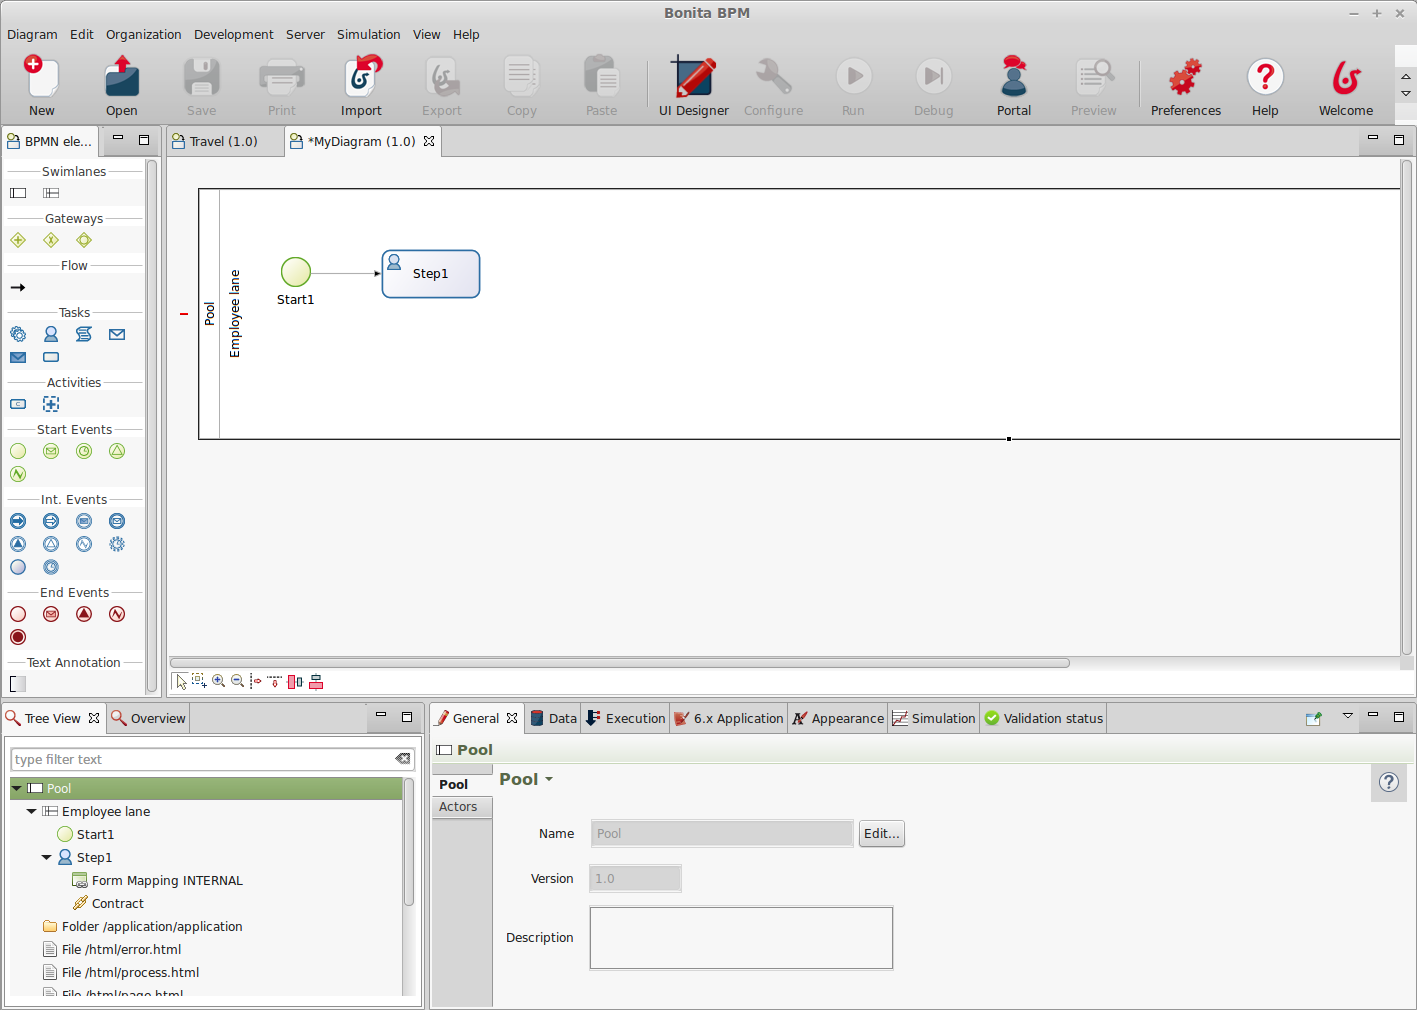
\includegraphics[width=1\textwidth]{images/bonita.png}
	\caption{Bonita BPM Interface}
	\label{fig:analyse:bonita:interface}
\end{figure}
Zuoberst ist die Toolbar. Darunter auf der linken Seite sind die BPMN Elemente (siehe \cref{sec:Recherche:bpmn:notation} \nameref{sec:Recherche:bpmn:notation}) wie z.B. die Swimlanes, Gateways und Events. Daneben kann der Prozess definiert werden in der Process View. Bei einem neuen Projekt hat es einen Start Event (mit dem Namen "`Start1"') und ein Task "`Step1"'. Bei dem Task hat es links oben ein Benutzer Icon. Dieses sagt aus, dass es sich um einen Human Task handelt, bei welchem eine Benutzerinteraktion benötigt wird.

Zuunterst links ist eine Übersicht über alle Elemente im Projekt (Tree View) und daneben können die BPMN Elemente im Projekt konfiguriert werden (Configuration View).

Bonita BPM ist mit Java implementiert. Auch die Erweiterungen (siehe \cref{sec:analyse:bonita:connectors} \nameref{sec:analyse:bonita:connectors}) werden in dieser Sprache entwickelt. Für das Verständnis wird vorausgesetzt, dass man grundlegendes Wissen für Java Begriffe besitzt (z.B. Namespace, Class, Implementation, Interface, etc.).

\subsection{Business Data Model}
\gls{bdm} werden für die Modellierung der Daten benötigt. Connectoren können später diese Daten entgegen nehmen oder zurückgeben. Intern handelt es sich dabei um Java Classes.

Ein \gls{bdm} hat einen Namen und Felder. Felder haben wiederum einen Namen und einen Java Datentypen (string, int oder ein weiteres \gls{bdm}). Ein Feld kann zusätzlich noch die zwei Attribute Multiple oder Mandatory haben. Ist Multiple gesetzt, so handelt es sich bei dem Feld um eine Liste, und Mandatory macht es zwingend, dass bei der Erstellung ein Wert zugewiesen wird.

\begin{figure}[H]
	\centering
	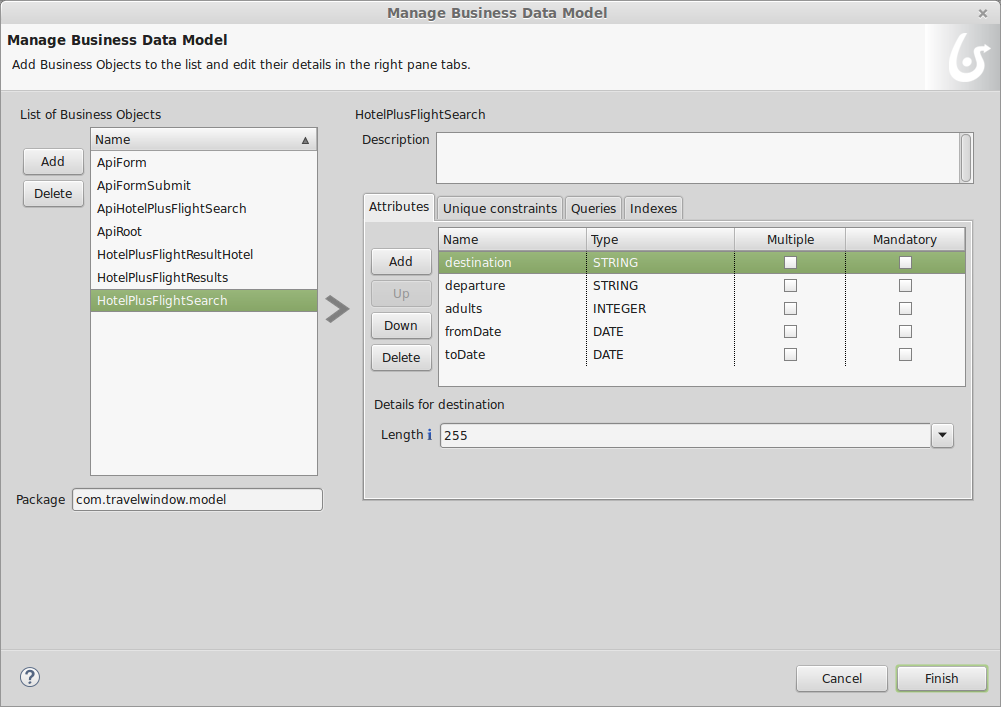
\includegraphics[width=0.8\textwidth]{images/bonita-bpm.png}
	\caption{Bonita BPM Business Data Model}
	\label{fig:analyse:bonita:bpm}
\end{figure}

\subsubsection{Pool Variables}
Ist in der Process View ein Pool angewählt, so kann in der Configuration View unter "`Data -> Pool Variables"' neue Pool Variablen definiert werden. Diese sind für alle Tasks in diesem Pool und Swimplanes sichtbar und können von den Connectors verwendet werden. Dabei handelt es sich um Instanzen von \glspl{bdm}. Eine Pool Variable besteht aus einem Namen, einem \gls{bdm} und einem Initialisierungs-Skript, um die Mandatory Fields abzufüllen.
\begin{figure}[H]
	\centering
	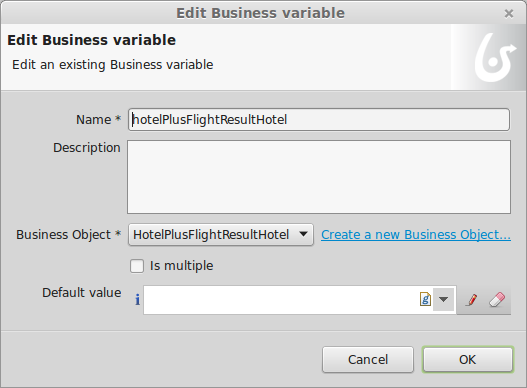
\includegraphics[width=0.8\textwidth]{images/bonita-poolvariables.png}
	\caption{Bonita BPM Pool Variables}
	\label{fig:analyse:bonita:bpm:poolvariables}
\end{figure}

\subsection{Connectors}
\label{sec:analyse:bonita:connectors}
Connectors werden in Bonita BPM dazu verwendet, um eine Aktion durchzuführen. 

Follgende Connectoren werden mit der Software ausgeliefert:
\begin{itemize}
\item CMS
\item CRM
\item Calendar
\item Database
\item ERP
\item LDAP
\item Messaging
\item Reporting
\item SOAP Web Services
\item Script
\item Social
\item Talend
\end{itemize}

Connectors werden einem Prozess angehängt. Klickt man einen Task in der Process View an, kann man in der Configuration View unter Execution Connectors hinzufügen.
\begin{figure}[H]
	\centering
	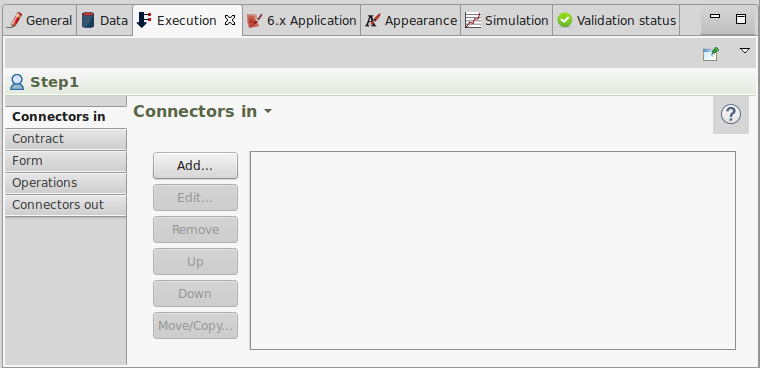
\includegraphics[width=1\textwidth]{images/bonita-connectors.png}
	\caption{Bonita BPM Connectors}
	\label{fig:analyse:bonita:connectors}
\end{figure}
Es gibt in und out Connectors. Diese werden entweder vor dem Task, oder nach dem Task ausgeführt. Bei einem Human Task kann so definiert werden, ob der Connector vor der Benutzerinteraktion ausgeführt wird oder danach.

Ein Connector besteht aus einer Definition und einer Implementation, welche nachfolgend beschrieben sind. In der Definition ist spezifiziert, was die Eingaben und Ausgaben sind. Wird ein Connector einem Task angehängt, so müssen die Eingaben definiert sowie ein Mapping der Ausgabeparameter gemacht werden.

\subsubsection{Definition}
Die Definition eines Connectors besteht aus Beschreibungsdaten (Name, Namespace, Kategorie, etc.), Input-Parameter, Wizard Pages und Output-Parameter. Als Input- und Output-Parameter können Java Classes oder \glspl{bdm} definiert werden. Wizard Pages werden dazu benötigt, dass wenn ein Connector einem Task hinzugefügt wird die entsprechenden Input-Parameter definiert werden können.

\subsubsection{Implementation}
Um eine Implementation eines Connectors anzulegen, muss zuerst eine Definition gewählt und Beschreibungsdaten angeben werden.
\begin{figure}[H]
	\centering
	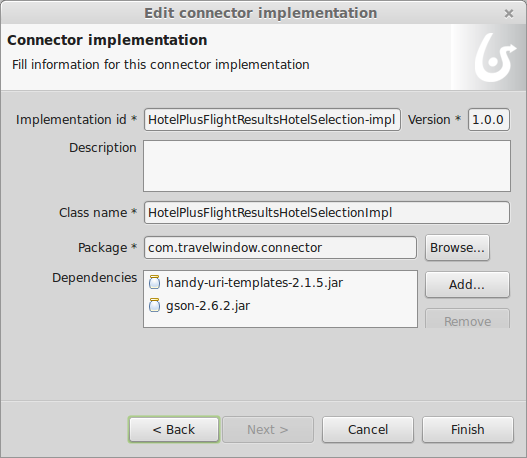
\includegraphics[width=1\textwidth]{images/bonita-connectors-implementation.png}
	\caption{Bonita BPM Connector Implementation}
	\label{fig:analyse:bonita:connectors:implementation}
\end{figure}
Die Implementation id kann frei gewählt werden, muss im Projekt jedoch eindeutig sein. Der Class name ist der Name der Java Klasse die erstellt wird. Dependencies sind JAR Files welche von innerhalb der Java Klasse benötigt werden.

Bestätigt man den obigen Dialog, so wird eine Java Klasse und abstrakte Klasse erzeugt. Nach dem obigen Beispiel werden die beiden Classes HotelPlusFlightResultsHotelSelectionImpl und AbstractHotelPlusFlightResultsHotelSelectionImpl erstellt. Das Hauptmethode der ersteren ist die Methode executeBusinessLogic. In der Definition dieses Connectors wurde definiert, dass ein \gls{bdm} HotelPlusFlightResultHotel zurückgegeben wird, welches den namen "`selection"' hat. Deshalb muss die Methode executeBusinessLogic die Methode "`setSelection"' aufrufen und dieser eine Classe vom Typen HotelPlusFlightResultHotel übergeben, um der Definition zu genügen. 
Die Methode setSelection ist dabei in der AbstractHotelPlusFlightResultsHotelSelectionImpl definiert.

Die Funktionalität eines Connectors kann somit frei implementiert werden. Zwingend ist nur das die Methode setSelection aufgerufen wird, sonst die die Ausführung des Connectors fehlerhaft.

\subsection{Forms, Contracts und Operations}
\label{sec:analyse:bonita:forms}
Bei einem Human Task muss ein Form angehängt werden, um dem Benutzer eine Interaktion in dem Prozess zu ermöglichen.
In einem Task kann direkt ein neues Formular erstellt werden. Es empfiehlt sich jedoch, zuerst den Contract zu definieren, da die dort angegeben Informationen automatisch bei der Erstellung des Forms und den Operations mitberücksichtigt werden. Weitere Informationen dazu werden den folgenden beiden Abschnitten gegeben.

\subsubsection{Contract}
\label{sec:analyse:bonita:forms:contract}
Ein Contract definiert die Daten, die vom Formular erwartet werden. Sie sind dafür verantwortlich, welche Informationen aus dem Process an das Form übergeben werden. Die dort definierten Werte können Java Klassen oder \glspl{bdm} sein. Beim Task für die Auswahl eines Hotels in der Hotel und Flug suche, könnte dies die Liste der Hotelresultate sein. Dazu wird im Contract eine Liste von Hotels angegeben.
\begin{figure}[H]
	\centering
	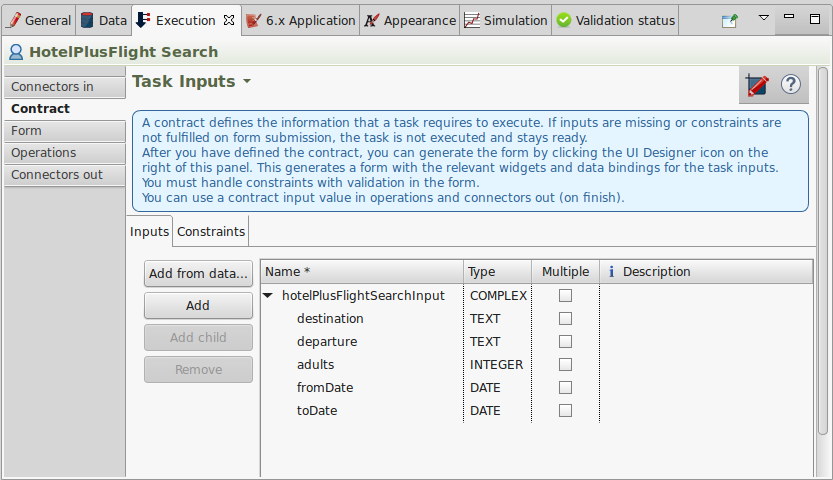
\includegraphics[width=1\textwidth]{images/bonita-contract.png}
	\caption{Bonita BPM Form Contract}
	\label{fig:analyse:bonita:forms:contract}
\end{figure}

\subsubsection{Operations}
\label{sec:analyse:bonita:forms:operations}
Operations werden nach der Ausführung des Formulars ausgeführt. Sie definieren, wie die Informationen aus dem Formular zurück in den Prozess fliessen.

\begin{figure}[H]
	\centering
	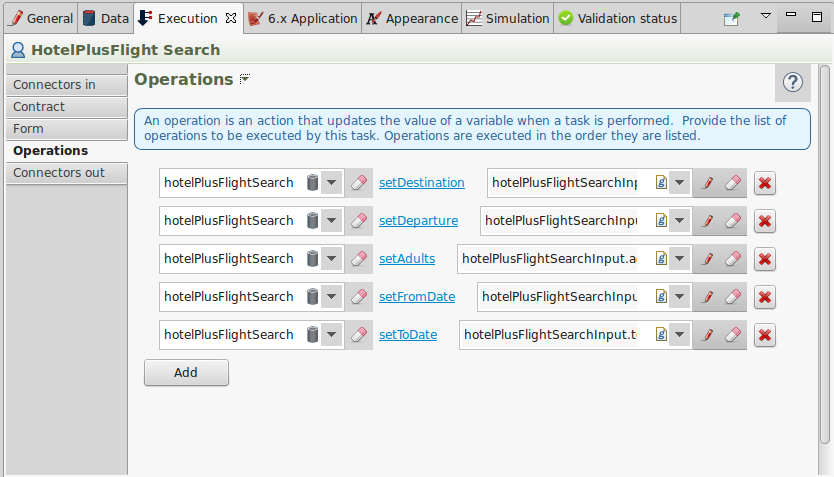
\includegraphics[width=1\textwidth]{images/bonita-operations.png}
	\caption{Bonita BPM Form Operations}
	\label{fig:analyse:bonita:forms:operations}
\end{figure}
Im obigen Beispiel wird definiert, dass auf der Pool Variable hotelPlusFlightSearch die Java Methode setDestination aufgerufen wird. Der Methode wird der Wert hotelPlusFlightSearchInput.destination übergeben. Bei hotelPlusFlightSearchInput handelt es sich um eine Variable, welche auf dem Formular definiert wurde (siehe \nameref{sec:analyse:bonita:forms:forms}).

\subsubsection{Forms}
\label{sec:analyse:bonita:forms:forms}
Ein Form ermöglicht die Interaktion eines Benutzers. Die Daten die an das Form übergeben werden und wie die bearbeiteten Daten zurück in den Process fliessen, ist in dem Contract und den Operations definiert (siehe \nameref{sec:analyse:bonita:forms:contract} und  \nameref{sec:analyse:bonita:forms:operations}). Es ist zu empfehlen, dass zuerst diese beiden Informationen definiert werden, da sie bei der Erstellung des Forms direkt weiterverwendet werden. Definiert man bei dem Contract dass eine Liste von Hotels übergeben wird, so wird bei der Erstellung des Formulars automatisch eine Liste generiert welche diese Daten anzeigt. 

Um ein Formular aus den Daten des Contracts und der Operations zu erstellen, muss dieses in der Configuration View erstellt werden.
\begin{figure}[H]
	\centering
	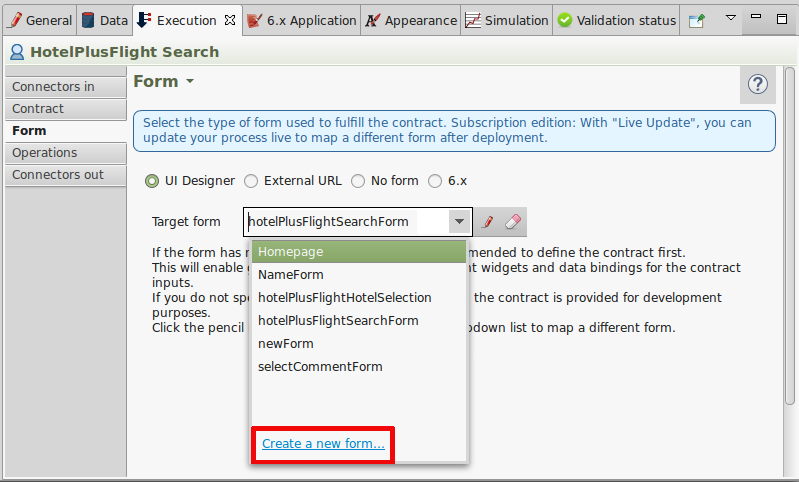
\includegraphics[width=1\textwidth]{images/bonita-forms-create.png}
	\caption{Bonita BPM Form erstellung aus Contract und Operations}
	\label{fig:analyse:bonita:forms:forms:creation}
\end{figure}

Danach öffnet sich der UI Designer. Dies ist ein Webinterface, welches auf dem mitgelieferten Tomcat Webserver läuft. Dort kann das Formular angepasst werden.
Die Funktionalität des UI Designers ist gross. Einen guten Überblick bietet ein Video Tutorial, welches von Bonitasoft bereit gestellt wird und auf folgender URL eingesehen werden kann \url{http://www.bonitasoft.com/resources/videos/getting-started-tutorial}. Ab 35:55 wird der UI Designer vorgestellt.